\documentclass[aspectratio=169, 10pt]{beamer}

% ---------------------------------------------------------------------------
% Pitch of empirical_strategy.tex to coauthors, built up to the predicted
% event-study picture: design in one picture -> prediction -> assignment ->
% estimation -> is it noise (the question slide is commented out). The
% backup opens with a linked overview, then follows the main deck: threats
% table, distance profile and comparison groups, mobility/2SLS, parametric
% spec, other estimands and checks, positioning in the literature.
% ---------------------------------------------------------------------------

\usetheme{metropolis}
\metroset{progressbar=frametitle, numbering=fraction}
\setbeamertemplate{navigation symbols}{}
\usepackage{appendixnumberbeamer}
\usepackage{amsmath}
\usepackage{amssymb}
\usepackage{tikz}
\usepackage{array}
\usepackage{booktabs}
\usepackage[style=authoryear, backend=biber, maxcitenames=2, uniquename=false, uniquelist=false]{biblatex}
\addbibresource{../Noise Pollution.bib}
\addbibresource{empirical_strategy_additions.bib}

\setbeamerfont{itemize/enumerate subbody}{size=\small}
\newcommand{\muted}[1]{{\color{black!55}#1}}
\newcolumntype{L}[1]{>{\raggedright\arraybackslash}p{#1}}
% Linked slide title on the backup overview.
\newcommand{\bklink}[2]{\hyperlink{#1}{\textcolor{mDarkTeal}{\textbf{#2}~$\rightarrow$}}}
% Return button in the bottom-left corner of each backup slide.
\newcommand{\backtooverview}{%
  \begin{tikzpicture}[remember picture, overlay]
    \node[anchor=south west, inner sep=0pt] at ([xshift=0.35cm, yshift=0.25cm]current page.south west)
      {\tiny\hyperlink{bk-overview}{\beamerreturnbutton{Overview}}};
  \end{tikzpicture}}

\begin{document}

% ---------------------------------------------------------------------------
% \begin{frame}{Does noise at home hold children back at school?}
% \small
% \textbf{Question.} Does living with road or rail noise during childhood lower grade-9 scores, and at which ages does it matter?
%
% \medskip
% \textbf{Why noise barriers.} Trafikverket has built hundreds of road and rail barriers over three decades. Each one cuts noise sharply on one side of the road, in a known year, and leaves the other side as it was.
%
% \medskip
% \textbf{Why Swedish registers.} Every child has a grade-9 score and is linked to their mother, whose residence is recorded each year on a 100\,m grid. We can place a family before the barrier and follow the child after the family moves.
% \end{frame}

% ---------------------------------------------------------------------------
\begin{frame}{The design in one picture}
\footnotesize
\begin{columns}[T]
\begin{column}{0.5\textwidth}
\centering
\textbf{Where: one corridor per barrier}\\[0.6em]
\begin{tikzpicture}[font=\scriptsize]
  % outer band
  \fill[mLightGreen!12] (0.8,2.45) rectangle (4.8,3.05);
  \draw[dashed, black!45] (0.8,2.45) rectangle (4.8,3.05);
  \node at (2.8,2.75) {600--1,500\,m behind: control 2};
  \node[black!45] at (2.8,2.12) {$\vdots$};
  % protected zone
  \fill[mLightGreen!40] (0.8,0.45) rectangle (4.8,1.75);
  \node at (2.8,1.1) {\textbf{protected} ($P=1$)};
  % barrier
  \draw[line width=2.5pt, mDarkTeal] (0.8,0.28) -- (4.8,0.28);
  \draw[mDarkTeal] (4.85,0.32) -- (5.15,0.9);
  \node[right, align=left, text=mDarkTeal] at (5.1,1.05) {barrier\\built $\tau_b$};
  % road
  \draw[thick, black!70] (0.4,0) -- (5.4,0);
  \draw[thick, black!70] (0.4,-0.12) -- (5.4,-0.12);
  \node[right, black!70] at (5.4,-0.06) {road / track};
  % opposite side
  \fill[black!10] (0.8,-0.4) rectangle (4.8,-1.7);
  \node[align=center] at (2.8,-1.05) {opposite side, same distance\\\textbf{main control}};
  % distance bands
  \draw[<->, black!55] (0.6,0.45) -- (0.6,1.75) node[midway, left] {$r$};
  \draw[<->, black!55] (0.6,-0.4) -- (0.6,-1.7) node[midway, left] {$r$};
\end{tikzpicture}
\end{column}
\begin{column}{0.48\textwidth}
\centering
\textbf{When: birth cohorts around $\tau_b$}\\[0.6em]
\begin{tikzpicture}[x=0.118cm, y=0.48cm, font=\scriptsize]
  \draw[->, black!70] (-22,0) -- (20,0) node[right] {year};
  \draw[dashed, mDarkTeal] (0,-0.2) -- (0,4.6);
  \node[below, text=mDarkTeal] at (0,-0.2) {$\tau_b$};
  \draw[dotted, black!60] (-3,-0.2) -- (-3,4.6);
  \node[below] at (-3.6,-0.2) {$\rho_b$};
  % cohort tested before the barrier
  \draw[line width=3pt, black!30] (-20,4) -- (-4,4);
  % cohort with dose 6
  \draw[line width=3pt, black!30] (-10,3) -- (0,3);
  \draw[line width=3pt, mLightBrown] (0,3) -- (6,3);
  % cohort with dose 13
  \draw[line width=3pt, black!30] (-3,2) -- (0,2);
  \draw[line width=3pt, mLightBrown] (0,2) -- (13,2);
  % cohort born after the barrier
  \draw[line width=3pt, mLightBrown!50] (1.2,1) -- (2,1);
  \draw[line width=3pt, mLightBrown] (2,1) -- (18,1);
  \foreach \y/\t in {4/-4, 3/6, 2/13, 1/18} \fill (\t,\y) circle (2.2pt);
  \node[right] at (19.5,4) {placebo};
  \node[right] at (19.5,3) {dose 6};
  \node[right] at (19.5,2) {dose 13};
  \node[right] at (19.5,1) {16 + utero};
\end{tikzpicture}\\[0.3em]
\muted{Bar: birth to test ($\bullet$, age 16). Brown: years lived with the barrier.}
\end{column}
\end{columns}

\bigskip
\small
\textbf{Design:} difference-in-differences across birth cohorts \emph{within} each barrier. Children from protected cells against children from the opposite side of the same road, cohorts tested before against cohorts tested after. The mother's cell in $\rho_b$, before the project, decides $P$.
\end{frame}

% ---------------------------------------------------------------------------
\begin{frame}{The prediction: zero, ramp, plateau}
\footnotesize
\begin{columns}[T]
\begin{column}{0.58\textwidth}
\centering
\textbf{If home noise harms scores cumulatively}\\[0.5em]
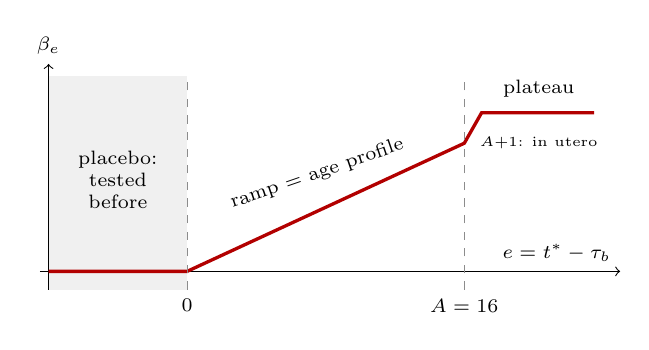
\begin{tikzpicture}[x=0.22cm, y=1.55cm, font=\scriptsize]
  \fill[black!6] (-8,-0.15) rectangle (0,1.6);
  \draw[->] (-8.5,0) -- (25,0) node[above left] {$e = t^* - \tau_b$};
  \draw[->] (-8,-0.15) -- (-8,1.7) node[above] {$\beta_e$};
  \draw[very thick, red!70!black] (-8,0) -- (0,0) -- (16,1.05) -- (17,1.3) -- (23.5,1.3);
  \draw[dashed, black!45] (0,-0.15) -- (0,1.6);
  \draw[dashed, black!45] (16,-0.15) -- (16,1.6);
  \node[below] at (0,-0.15) {$0$};
  \node[below] at (16,-0.15) {$A=16$};
  \node[align=center] at (-4,0.75) {placebo:\\tested\\before};
  \node[align=center, rotate=19] at (7.5,0.8) {ramp = age profile};
  \node[font=\tiny] at (20.3,1.05) {$A{+}1$: in utero};
  \node at (20.3,1.5) {plateau};
\end{tikzpicture}
\end{column}
\begin{column}{0.4\textwidth}
\begin{itemize}\setlength{\itemsep}{2pt}
  \item $e<0$: no exposure, $\beta_e = 0$
  \item Each later cohort adds one year, at a younger age: the step $\beta_e - \beta_{e-1}$ is the effect of exposure at age $A-e$
  \item $\beta_{A+1} - \beta_A$: exposure in utero
  \item Cohorts born after the barrier have the same dose: flat
\end{itemize}
\end{column}
\end{columns}

\medskip
\textbf{Other stories draw other pictures}\\[0.3em]
\begin{tabular}{@{}ccc@{}}
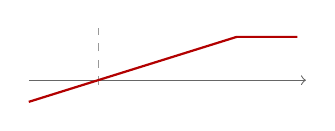
\begin{tikzpicture}[x=0.11cm, y=0.55cm]
  \draw[->, black!60] (-8,0) -- (24,0); \draw[dashed, black!40] (0,-0.1) -- (0,1.2);
  \draw[thick, red!70!black] (-8,-0.5) -- (0,0) -- (16,1) -- (23,1);
\end{tikzpicture}
&
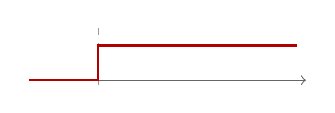
\begin{tikzpicture}[x=0.11cm, y=0.55cm]
  \draw[->, black!60] (-8,0) -- (24,0); \draw[dashed, black!40] (0,-0.1) -- (0,1.2);
  \draw[thick, red!70!black] (-8,0) -- (0,0) -- (0,0.8) -- (23,0.8);
\end{tikzpicture}
&
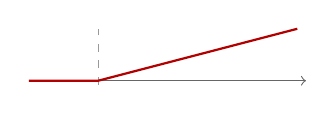
\begin{tikzpicture}[x=0.11cm, y=0.55cm]
  \draw[->, black!60] (-8,0) -- (24,0); \draw[dashed, black!40] (0,-0.1) -- (0,1.2);
  \draw[thick, red!70!black] (-8,0) -- (0,0) -- (23,1.2);
\end{tikzpicture}
\\[-0.2em]
\scriptsize\textbf{Pre-trend:} &
\scriptsize\textbf{Step, no ramp:} &
\scriptsize\textbf{No plateau:} \\[-0.3em]
\scriptsize sorting, anticipation &
\scriptsize noise around the test &
\scriptsize trends set off by the road project
\end{tabular}
\end{frame}

% ---------------------------------------------------------------------------
\begin{frame}{Who counts as exposed: the cell before the project}
\small
\textbf{Threat:} families move in, move out or stay \emph{because of} the barrier, and road projects are announced years ahead. Assigning by current address would build sorting into the ramp.

\medskip
\textbf{Assignment}
\begin{itemize}
  \item \textbf{Reference cell:} the mother's 100\,m cell on 31 December of $\rho_b$, before the project could affect where families live
  \item $\rho_b$ = year before the project was announced; with no project dates yet, $\rho_b = \tau_b - 3$ (robustness: $\tau_b - 1$, $\tau_b - 5$; later dates should give smaller estimates if anticipation matters)
  \item Through the mother, children born after $\tau_b$ get a cell by the same rule as their older siblings
  \item Children are followed after moves: an \textbf{intention-to-treat} effect. Moving becomes a mechanism, not a threat
\end{itemize}

\medskip
\textbf{Not:} stayers only \parencite[as][]{lindgrenSoundEnvironmentHealth2021}, which selects on a response to treatment; or dwellings \parencite[as][]{morettiTrafficNoiseExternality2025}, which mixes the effect with who moves in and out.
\end{frame}

% ---------------------------------------------------------------------------
\begin{frame}{Estimation: one stack per barrier}
\footnotesize
\vspace{-0.4em}
\[
S_i = \sum_{e \neq -1} \beta_e\, \mathbf{1}\{e_i = e\}\, P_i + \gamma_{b,P_i,r(i)} + \eta_{b,e_i} + X_{f(i)}'\phi + \varepsilon_i
\]
\vspace{-1.2em}
\begin{columns}[T]
\begin{column}{0.49\textwidth}
\begin{itemize}\setlength{\itemsep}{1pt}
  \item $S_i$: grade-9 merit value as a percentile within the test year (grading changed over time)
  \item $\gamma_{b,P,r}$: each side \texttimes{} distance band, per barrier
  \item $\eta_{b,e}$: barrier \texttimes{} test year. Absorbs traffic, local shocks and the road project as far as it is the same at all distances. Robustness: $\eta_{b,r,e}$, same distance band only
  \item $X_{f(i)}$: parental education, income, immigrant background at $\rho_b$
  \item No school FE (school chosen after $\tau_b$); robustness: \emph{assigned} school \texttimes{} test year
  \item Event time and dose from the \emph{intended} test year $t^* = a_i + 16$, so repeating a grade does not change them
\end{itemize}
\end{column}
\begin{column}{0.49\textwidth}
\begin{itemize}\setlength{\itemsep}{1pt}
  \item Each barrier is compared only with its own cells; cells protected by another barrier are dropped \parencite{cengizEffectMinimumWages2019}
  \item Weighted by protected children, event study on barriers with a full window (built by about 2007) \parencite{wingStackedDifferenceinDifferences2024}
  \item Clustered by connected corridors; wild cluster bootstrap and randomisation inference
  \item \textbf{Headline:} effect per year of assigned dose, once pre-trends are flat and the ramp is roughly linear
  \item Cross-checks: \textcite{callawayDifferenceinDifferencesMultipleTime2021}, \textcite{sunEstimatingDynamicTreatment2021}, \textcite{borusyakRevisitingEventStudyDesigns2024}
\end{itemize}
\end{column}
\end{columns}
\end{frame}

% ---------------------------------------------------------------------------
\begin{frame}{Is it the noise?}
\small
Road barriers come with a road project and lower near-road air pollution \parencite{baldaufImpactsNoiseBarriers2008,greenhillNoisePollutionInfant2026}. Three tests separate noise from the bundle:

\renewcommand{\arraystretch}{1.1}
\footnotesize
\begin{tabular}{@{}L{0.29\textwidth}L{0.3\textwidth}L{0.35\textwidth}@{}}
\toprule
\textbf{Test} & \textbf{If it is noise} & \textbf{If it is the project or air pollution} \\
\midrule
\textbf{Rail against road} & Similar ramps: rail traffic is mostly electric, so a rail barrier changes little but noise & Ramp for road barriers only \\
\textbf{Threshold}, fixed in advance: $L^0$ above WHO guideline (53\,dB road, 54\,dB rail) & Ramp above the threshold, none below & Ramp below the threshold too, among cells as close to the road (same project) but quiet to begin with \\
\textbf{Intensity}: predicted dB the barrier removes at each cell & Larger ramp where the barrier removes more dB & Same ramp whatever the dB cut \\
\bottomrule
\end{tabular}

\smallskip
\muted{Threshold and intensity compare cells at the same distance from the road: the project's effects also fade with distance.}
\end{frame}

% ===========================================================================
\appendix
\begin{frame}[standout]
  Backup
\end{frame}

% ---------------------------------------------------------------------------
\begin{frame}[label=bk-overview]{Backup: overview}
\footnotesize
\renewcommand{\arraystretch}{1.35}
\begin{tabular}{@{}L{0.33\textwidth}L{0.42\textwidth}L{0.17\textwidth}@{}}
\toprule
\textbf{Slide} & \textbf{What it covers} & \textbf{Backs up} \\
\midrule
\bklink{bk-threats}{Threats and answers} & Each threat, the design answer and the evidence we show & All \\
\bklink{bk-distance}{Distance and comparison groups} & The three comparison groups; effect by 50\,m bin; balance before the barrier & Design \\
\bklink{bk-mobility}{Mobility and per year lived} & Moving as a mechanism; 2SLS on years actually lived & Assignment \\
\bklink{bk-dose}{Dose and age profile} & Parametric effect per year of dose; kinks by age; duration against intensity & Prediction, estimation \\
\bklink{bk-checks}{Other estimands and checks} & Siblings, residents at the test, heterogeneity, placebo checks & Threats \\
\bklink{bk-literature}{Literature} & What we take from each study and what we do differently & Contribution \\
\bklink{bk-references}{References} & & \\
\bottomrule
\end{tabular}
\end{frame}

% ---------------------------------------------------------------------------
\begin{frame}[label=bk-threats]{Backup: threats and answers}
\footnotesize
\renewcommand{\arraystretch}{1.3}
\begin{tabular}{@{}L{0.27\textwidth}L{0.35\textwidth}L{0.32\textwidth}@{}}
\toprule
\textbf{Threat} & \textbf{Design answer} & \textbf{Evidence we show} \\
\midrule
Families sort or anticipate & Reference cell at $\rho_b$, via the mother; ITT & Mobility event study; births by side; predicted-score placebo \\
Road project comes with the barrier & Opposite side of the same road; barrier \texttimes{} year FE & Threshold, intensity, plateau; barrier \texttimes{} band \texttimes{} year FE \\
Air pollution moves with noise & Rail against road & NO\textsubscript{2} by side, if a grid exists \\
Staggered timing, bad comparisons & Stacking, own cells only, corrective weights & Callaway--Sant'Anna, Sun--Abraham, Borusyak et al. \\
Cells misclassified at the zone edge & Drop edge cells (100\,m grid) & Estimates with them included \\
Comparison cells insulated & --- (bias toward zero) & Insulation records, if they exist \\
Grading changes & Percentile within test year & Raw merit value, national tests \\
Sides feed different schools; grading by school & Assigned school \texttimes{} year FE (not actual school: post-treatment) & School overlap of the two sides; actual school \texttimes{} year FE as decomposition \\
\bottomrule
\end{tabular}
\backtooverview
\end{frame}

% ---------------------------------------------------------------------------
\begin{frame}[label=bk-distance]{Backup: distance profile and comparison groups}
\footnotesize
\begin{itemize}
  \item \textbf{Comparison groups:} (1) opposite side, same distance (main); (2) 600--1,500\,m behind the barrier; (3) not-yet-treated corridors (robustness). Not never-treated places alone: places eligible but never shielded may have low priority for reasons that also shape their trends
  \item \textbf{Caveat for (1):} the unshielded side may lack a barrier because it has few dwellings or got insulation, which we check
  \item \textbf{Distance profile:} the effect in 50\,m bins of distance from the barrier up to 1,500\,m, each against the opposite side at the same distance. Shows how far the protection reaches, and whether the 600--1,500\,m band is unaffected; if not, the band moves out
  \item \textbf{Balance:} for cohorts tested before the barrier, scores should vary with distance in the same way on both sides \parencite{berkhoutLeadExposureCognitive2025}
\end{itemize}
\backtooverview
\end{frame}

% ---------------------------------------------------------------------------
\begin{frame}[label=bk-mobility]{Backup: mobility and the effect per year lived}
\footnotesize
\[
M_{ft} = \sum_{k \neq -1} \mu_k\, \mathbf{1}\{t - \tau_b = k\}\, P_f + \gamma_{b,P_f,r(f)} + \eta_{b,t} + X_f'\phi + u_{ft}
\]
\begin{itemize}
  \item \textbf{Mobility as mechanism:} hazard of leaving the reference cell. Moves between $\rho_b$ and $\tau_b$ indicate anticipation
  \item \textbf{Per year lived:} 2SLS with years actually lived behind a barrier, instrumented by the assigned dose: an average causal response among compliers \parencite{angristTwoStageLeastSquares1995}
  \item A \emph{LATE} if the barrier does not change moving or schools, else a \emph{rescaled ITT}; bounds that allow a direct effect of assignment \parencite{conleyPlausiblyExogenous2012}
  \item Compliers described by household characteristics at $\rho_b$ \parencite{abadieSemiparametricInstrumentalVariable2003}
\end{itemize}
\backtooverview
\end{frame}

% ---------------------------------------------------------------------------
\begin{frame}[label=bk-dose]{Backup: effect per year of dose and age profile}
\footnotesize
\[
S_i = \beta\, D_i P_i + \beta^{\text{utero}}\, \mathbf{1}\{e_i > A\}\, P_i + \beta^{\text{pre}}\, \mathbf{1}\{e_i < 0\}\, e_i\, P_i + \gamma_{b,P_i,r(i)} + \eta_{b,e_i} + X_{f(i)}'\phi + \varepsilon_i
\]
\[ D_i = \min\{\max(0,\, e_i),\, A\} \]
\begin{itemize}
  \item $\beta$: effect per year of assigned dose; $\beta^{\text{utero}}$: added effect of exposure in pregnancy; $\beta^{\text{pre}}$: pre-trend test
  \item Age profile: slope allowed to differ by the age of the added year, kinks at 3, 7 and 13
  \item Not a regression on $D_i$ alone: cohorts tested before would pool with comparison cells and the placebo would be lost; a continuous dose with staggered timing needs stronger parallel trends \parencite{callawayDifferenceinDifferencesContinuousTreatment2024}
  \item Duration against intensity: years of exposure holding dB-years $D_i \Delta L$ fixed \parencite{hollingsworthThousandCutsCumulative2025}; permutation of $\Delta L$ within corridors
\end{itemize}
\backtooverview
\end{frame}

% ---------------------------------------------------------------------------
\begin{frame}[label=bk-checks]{Backup: other estimands and checks}
\footnotesize
\begin{columns}[T]
\begin{column}{0.49\textwidth}
\textbf{Other estimands}
\begin{itemize}\setlength{\itemsep}{1pt}
  \item \textbf{Siblings:} household fixed effects with birth order \texttimes{} sex fixed effects \parencite{blackMoreMerrierEffect2005}; selected toward large families that stay, so robustness only
  \item \textbf{Residents at the test:} the dwelling-based estimand; its gap to the ITT measures sorting; compositional-change test \parencite{santannaDifferenceinDifferencesCompositionalChanges2025}
\end{itemize}
\textbf{Heterogeneity, fixed in advance}
\begin{itemize}\setlength{\itemsep}{1pt}
  \item Sex; parental education, income, immigrant background; housing type
  \item Wind direction: heterogeneity by side only, since it carries pollution too
\end{itemize}
\end{column}
\begin{column}{0.49\textwidth}
\textbf{Checks}
\begin{itemize}\setlength{\itemsep}{1pt}
  \item Predicted score from household characteristics at $\rho_b$ as a placebo outcome
  \item Births after $\rho_b$: number and mothers' characteristics by side
  \item $\tau_b$ shifted back five years
  \item Off-age testing by $P_i$ after $\tau_b$; children tested on time only
  \item Dated against undated barriers: location, length, road type, neighbourhood
  \item Birth outcomes for cohorts born after $\tau_b$ (access to be confirmed)
\end{itemize}
\end{column}
\end{columns}
\backtooverview
\end{frame}

% ---------------------------------------------------------------------------
\begin{frame}[label=bk-literature]{Backup: how this relates to the literature}
\footnotesize
\renewcommand{\arraystretch}{1.3}
\begin{tabular}{@{}L{0.3\textwidth}L{0.3\textwidth}L{0.34\textwidth}@{}}
\toprule
\textbf{Study} & \textbf{We take} & \textbf{We do differently} \\
\midrule
\textcite{lindgrenSoundEnvironmentHealth2021}: Swedish noise mitigation and health & The setting & Keep movers; same-road controls, not never-treated \\
\textcite{morettiTrafficNoiseExternality2025}: barriers and house prices & The 600--1,500\,m band & Follow people, not dwellings; no unbuilt barriers in Sweden \\
\textcite{greenhillNoisePollutionInfant2026}: noise and infant health & Noise and air pollution move together & Rail as a near noise-only treatment \\
\textcite{gronqvistUnderstandingHowLow2020}: lead, Swedish cohorts & Cohort \texttimes{} exposure, threshold fixed in advance, percentile outcome & Place-specific timing; dose from years lived \\
\textcite{hollingsworthThousandCutsCumulative2025}; \textcite{berkhoutLeadExposureCognitive2025} & Duration against intensity; age profile; distance cut-off from the data & Noise, not lead \\
\bottomrule
\end{tabular}

\medskip
\small
\textbf{What we add:} a cohort exposure design for noise and school achievement, with assignment before the barrier and a within-corridor comparison that nets out the road project.
\backtooverview
\end{frame}

% ---------------------------------------------------------------------------
% No label= here: it stops allowframebreaks from breaking, cutting the list.
\begin{frame}[allowframebreaks]{References}
\hypertarget{bk-references}{}\scriptsize
\printbibliography[heading=none]
\end{frame}

\end{document}
